\documentclass[]{report}


\usepackage[autostyle]{csquotes} 
\usepackage{parskip}
\usepackage{graphicx}


% Title Page
\title{Context-aware framework}
\author{Jacob B. Cholewa \& Mathias Kindsholm Pedersen}


\begin{document}
\maketitle

\begin{abstract}
\end{abstract}


\chapter{Project description}
A Context-aware system is able to adapt its behavior to the surroundings it is in. In order to act upon its environment, the system will need sensor-input. Various sources of input can be used to determine the actions of the system.\\

In this project we want to mainly focus on implementing a context-awareness framework, making it easy for systems to actuate on sensor events. As a proof of concept we will explore replacing the physical SCRUM board, which is often a whiteboard and post-its, with an IT-solution which is not confined to a personal computer, but has the same presence. The digital SCRUM board will be context-aware to the extent that it can recognize different SCRUM activities, like sprint meeting or one-on-one, and automatically change its graphical interface.


\chapter{Scope}
Scoping of our project description - especially what we will NOT do

\chapter{Background research}


To be able to make a context-aware framework, we first had to investigate what context and context-awareness is in a computer science perspective.


When being face-to-face with a person people can interpret the situation and that is a very important factor in effective communication. 

When communication with computers they can not understand and interpret the situation and that leads to inefficient human-machine interaction. Context-aware computing can apply situation information to machines.

Context-awareness is a term associated with Ubiquitous computing also known as Pervasive computing.

Ubiquitous computing, ubicomp, was coined in the early nineties by Mark Weiser whose vision was to make technology that could seamlessly assist in everyday tasks. Weisers research-unit at Xerox PARC developed some of the first mobile devices, and the development of ubi computing clearly reflects in todays technology boom of smart phones and tablets.

Many of the publications on the subject describes it different, but the one description fitting best our understanding was coined by Dey and Abowd whom described context as:


\blockquote{
	Any information that can be used to characterize the situation of an entity. An entity is a person, place or object that is considered relevant to the interaction between a user and an application, including the suer and application themselves. \cite{Dey and Abowd (2000)} 
} 

We will in this project be focused on how we can effectively model situation in computer software.






  

\chapter{Design Choices}

This chapter describes the different design choices we have though about in developing the framework.


\section{Encapsulation of Context}

Extension with properties vs. composite
Situations


\section{Widget}

\section{Central}

Blackboard vs. Widget

\section{Client}


\section{Dynamic Entity types}


\section{Communication}

Multicasting




\chapter{Design}




\section{Overview}

\begin{center}
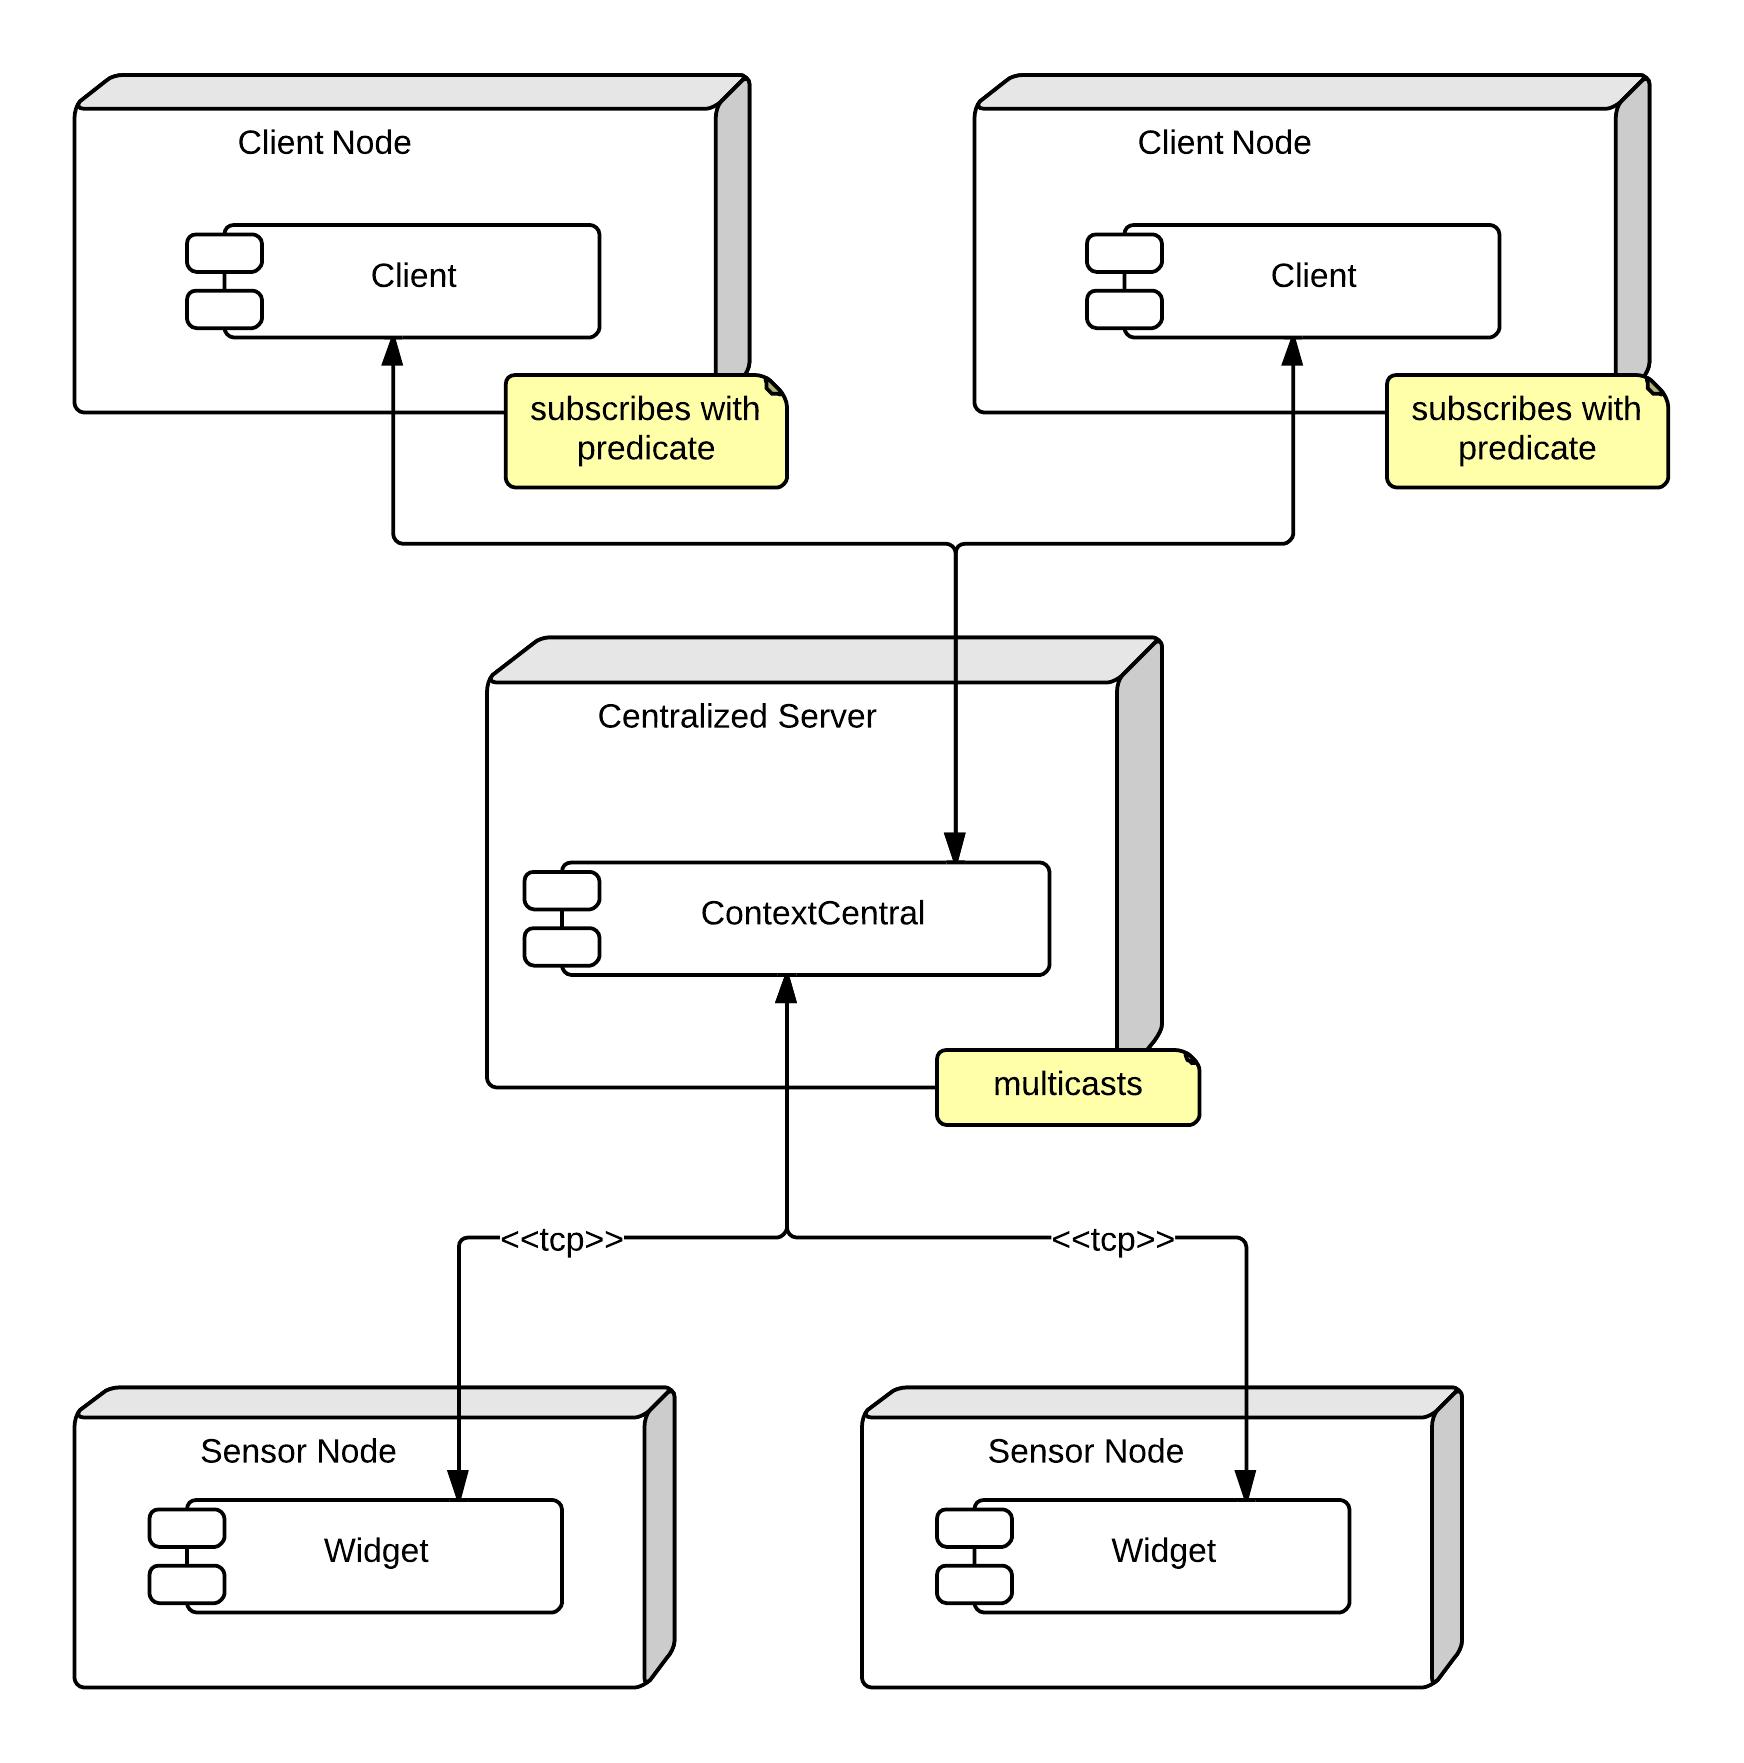
\includegraphics[scale=0.2]{ComponentDiagram.png}
\end{center}


\paragraph{The Client} is an observer interested in sensor data. It subscribes to a situation on the ContextCentral.

\paragraph{The Widget} wraps a sensor and translates the raw data to entities which are sent to the ContextCentral.

\paragraph{The ContextCentral} is the central for entity information and situations. When an entity is received from a widget, all stored situations are checked and subscribers notified accordingly.



\section{Encapsulation of Context}
Design choices in encapsulating context

Entities are generalized by the type IEntity, specifying general information for all entities.


\begin{center}
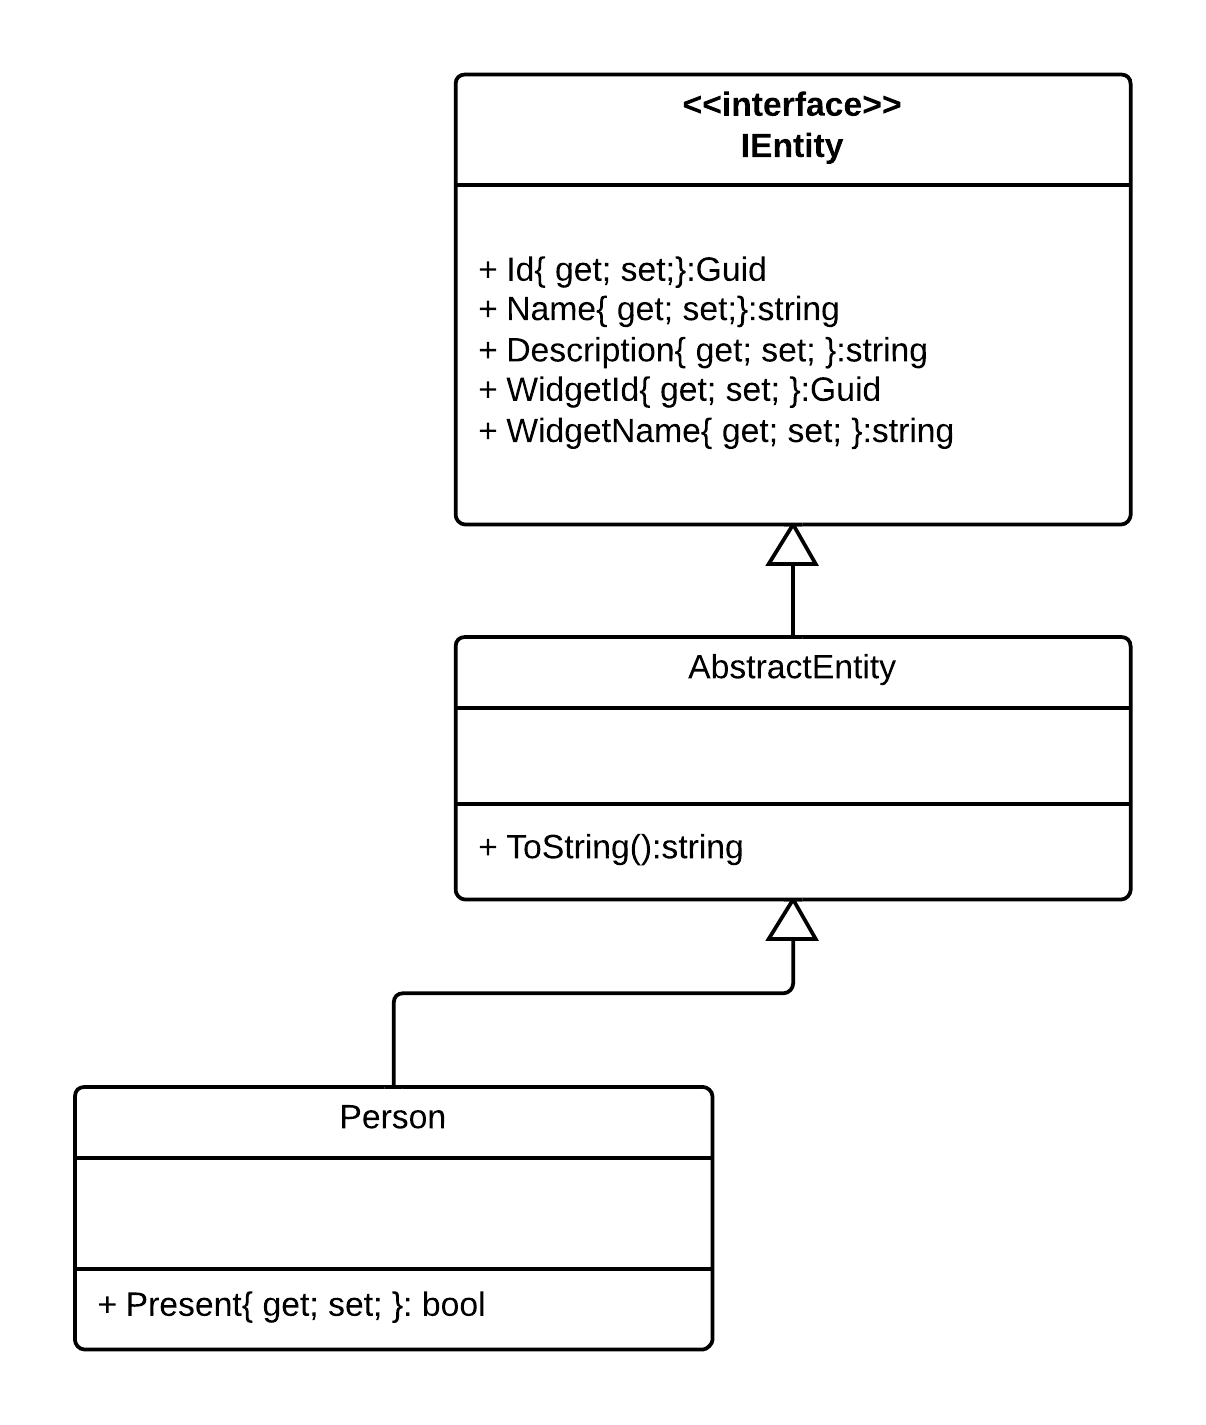
\includegraphics[scale=0.15]{ContextClassDiagram.png}
\end{center}


\section{Widget}

\section{Central}

\section{Client}

\section{Communication}


\chapter{Conclusion}

\begin{thebibliography}{9}

\bibitem{Dey and Abowd (2000)}
  Dey, A. K., and Abowd, G.D.
  \emph{Towards a better understanding of context and context-awareness. Workshop on the What, Who, Where, When and How Context-awareness, afflicted with the 2000 ACM Conference on Human Factors in Computer Systems},
  2000.

\end{thebibliography}
\chapter{Appendixes}

\end{document}
